\customHeader{1}{Evaluation Metrics for Classification}
\label{02_evaluation_metrics}

After training a classifier for a Classification task, including \textclassification{}, the subsequent phase is to assess its performance. 
This involves leveraging a dataset with predefined class labels and contrasting the classifier's \emph{predicted} with these \emph{true} labels.

In Binary Classification, we deal with two classes. Here, for simplicity, we  referred to them as the positive and negative classes. 
Our primary concern is to measure how well the positive class is predicted.
The primary focus here is to gauge the accuracy of positive class predictions. The content of this section is an adaptation of \mytextcite{fbetascore}.


When the classifier is applied to an item, there are four potential outcomes, contingent on the classifier's predictions and the true class labels. These four cases constitute a \emph{Confusion Matrix} (as depicted in Table \ref{tab:confusion_matrix}).





\begin{table}[ht]
\centering
\resizebox{\textwidth}{!}{
\begin{tabular}{ll}

\textbf{Case} & \textbf{Description} \\
True Positives (TP) & The item \emph{is} in the positive class, and the classifier \emph{predicts} the positive class. \\
True Negatives (TN) & The item \emph{is} in the negative class, and the classifier \emph{predicts} the negative class. \\
False Negative (FN) & The item \emph{is} in the positive class, and the classifier \emph{predicts} the negative class. \\
False Positive (FP) & The item \emph{is} in the negative class, and the classifier \emph{predicts} the positive class. \\
\end{tabular}
}
\caption{Classification Outcomes}
\label{tab:02_classification_outcomes}
\end{table}

\begin{table}[ht]
\centering
\resizebox{\textwidth}{!}{
    \begin{tabular}{|c|c|c|}
    \hline
    \textbf{Actual Class/Predicted Class} & \textbf{Predicted Positive} & \textbf{Predicted Negative} \\
    \hline
    \textbf{Actual Positive} & TP & FN \\
    \hline
    \textbf{Actual Negative} & FP & TN \\
    \hline
    \end{tabular}
}
\caption{Confusion Matrix for Binary Classification}
\label{tab:confusion_matrix}
\end{table}

There are four classic metrics for evaluating classifiers:

\begin{itemize}
    \item Accuracy: Accuracy measures the overall correctness of a classification model. It is the ratio of \emph{correctly} predicted instances to the total number of instances in the dataset.\\
    \begin{align}
    A &= \dfrac{TP + TN}{Positives + Negatives}  \label{eq:def_accuarcy}
\end{align}
    Example: If a model classifies 90 out of 100 samples correctly, the accuracy would be 90\%.
    
    \item Precision: Precision quantifies the ability of a model to correctly identify positive instances among the ones it predicted as positive. It is the ratio of true positive predictions to the total number of positive predictions (both true positives and false positives).
    \begin{align}
    P &= \dfrac{TP}{Predicted Positives} \\
        &=\dfrac{TP}{TP + FP}  \label{eq:def_precision}
    \end{align}
    
    Example: If a model predicts 100 instances as positive, and 80 of them are truly positive, the precision would be 80\%. 
    
    Note that, with a model that almost always predicts the negative class, there will be minimal False Positives and True Positives ($FP, TP \to 0$), and thus, this flawed model would have nearly 0\% precision.

    \item Recall (Sensitivity or True Positive Rate): Recall measures the ability of a model to correctly identify all positive instances in the dataset. It is the ratio of true positive predictions to the total number of actual positive instances in the dataset. 

    \begin{align}
    R   &= \dfrac{TP}{Actual Positives} \\
        &= \dfrac{TP}{TP + FN} \label{eq:def_recall}
    \end{align}

    Example: If there are 100 positive instances in the dataset, and the model correctly identifies 80 of them, the recall would be 80\%.

    Note that, with a model that almost always predicts the positive class, there will be minimal False Negatives ($FN \to 0$), and thus, this flawed model would have nearly 100\% recall.

    \item \fOne{} Score: The \fOne{} score is the harmonic mean of precision and recall. It balances the trade-off between precision and recall and provides a single metric to evaluate a model's performance.

    \begin{align}
    F_1 &= \left(\dfrac{1}{P} + \dfrac{1}{R}\right)^{-1} \label{eq:def_f1}\\
        &= 2 * \dfrac{P * R}{P + R}
    \end{align}


    Example: If a model has a precision of 75\% and recall of 80\%, the \fOne{} score would be calculated as $2 * ((0.75 * 0.80) / (0.75 + 0.80)) = 77, 4\%$.


    
\end{itemize}

Now that we have discussed the \fOne{} score, let's take a step further and introduce the \fBeta{} score. The \fBeta{} score extends the concept of \fOne{} by introducing a parameter $\beta$, which allows us to control the trade-off between precision and recall. A higher value of beta emphasizes recall, while a lower value emphasizes precision. The \fOne{} score is a special case of the \fBeta{} score when $\beta$ is set to 1.


\begin{align}
    F_\beta &= (1+\beta^2) \dfrac{P * R}{\beta^2* P + R} \label{eq:def_f_beta}
\end{align}


Example: If $\beta$ is set to $2$, the \fTwo{} score will give more two times more weight to recall than precision, making it suitable for tasks where recall is more important than precision, such as ours.

\putInBox{
Our task involves distinguishing between events representing health risks and impacting agriculture (the positive class) from harmless events (the negative class). In this context, it becomes vital to identify as many true positive cases as possible, as they represent actual risks with potential consequences for agriculture. We place a higher priority on this aspect, even if it leads to some harmless events being missclassified.
This is because, once our system flags a potential risk, subject experts will be notified to make the final assessment. As a result, our focus leans more towards improving recall over precision.
Therefore, we choose to assess our system using the \fTwo{} score.
}



\customHeader{2}{Evaluating Probabilistic Classifiers}
\label{02_evaluating_probabilistic_classifiers}

A probabilistic binary classifier is a classifier that produces likelihood of an item being in the positive class or negative class, rather than giving a definitive verdict. To take a decision, a specific threshold or cut-off is needed. For example, if a 50\% threshold is chosen for the positive class, items with probabilities above this are deemed positive, while those below are seen as negative. Additionally, this threshold can be adjusted to be more stringent, requiring a higher confidence level (e.g., 60\%) for positive classification, or more lenient, allowing lower confidence (e.g., 40\%) for positive classification, and so on \myparencite{auc_definition}.

When evaluating a probabilistic classifier using a labeled dataset, different thresholds lead to varied confusion matrices. Using this insight, we can formulate a metric to evaluate such classifiers. To do this, we first need to understand two key concepts:


\begin{itemize}
    \item The True Positive Rate ($TPR$) is the ratio of True Positive predictions to all actual Positive cases. That is, it's the recall (Equation \ref{eq:def_recall}). It assesses the classifier's efficacy with respect to the positive portion of the dataset.

    \begin{align}
        TPR &= \dfrac{TP}{TP+FN} =R \label{def_tpr} 
    \end{align}
    
    \item The False Positive Rate ($FPR$) is the ratio of False Positive predictions to all actual Negative cases. It assesses the classifier's efficacy concerning the negative portion of the dataset, but in a reverse manner. That is, a  higher $FPR$ means worse performance regarding the negatives, and lower $FPR$ means better performance (Equation  \ref{def_fpr_2}).
    
    \begin{align}
        FPR &= \dfrac{FP}{TN+FP} \label{def_fpr} \\
            &= 1 - \dfrac{TN}{TN+FP} \label{def_fpr_2}
    \end{align}
    
\end{itemize}

The fundamental observation is that selecting a particular probability threshold gives rise to specific values in the confusion matrix, which in turn provides a pair of values $(FPR, TPR)$. Plotting these points as the threshold varies creates the \emph{Receiver Operating Characteristic} (ROC) curve.

To introduce the \gls{auc} measure, let's further explore the nuances of the ROC curve (Refer to Figure \ref{fig:02_auc}):


\begin{enumerate}
    \item A threshold of 0\% implies that every item is classified as a positive, thus, there are no False Negatives and no True Negatives, which means that the FPR and TPR are both 1.

    \item A threshold of 100\% implies that every item is classified as a negative, thus, there are no True Positives and no False Positives, which means that the FRP and TPR are both 0.

    \item Combining these two observations, if we plot the curve by decreasing the threshold from 100\% to 0\%, we will obtain a curve starting from point $(0,0)$ and ending at point $(1,1)$.

    \item A perfect classification system would make no mistakes, no matter the probability threshold\footnote{Except for thresholds of 0\% and 100\%, as explained above}. That is, it would have no False Positives and no False Negatives. This would make the TPR always 1, which corresponds to a horizontal line 1 unit above the horizontal axis. 

    \item A completely inaccurate classification system is always wrong, no matter the probability threshold. That is, it would never have True Positives nor True Negatives. This would make the TPR always 0, which corresponds to a horizontal line on top of the horizontal axis.

    \item A classification system that always takes decisions at random, is equally likely to correctly identify positive instances as it is to incorrectly label negative instances as positive. This means, the $FPR$ and $TPR$ would always be equal, which corresponds to a diagonal line.

    \item A classification system that performs better than a random classifier will have a performance tending towards a perfect classifier, which corresponds to a curve above the diagonal.

    \item A classification system that performs worse than a random classifier will have a performance tending towards a completely inaccurate classifier, which corresponds to a curve below the diagonal.

\end{enumerate}

\begin{figure}
    \centering
    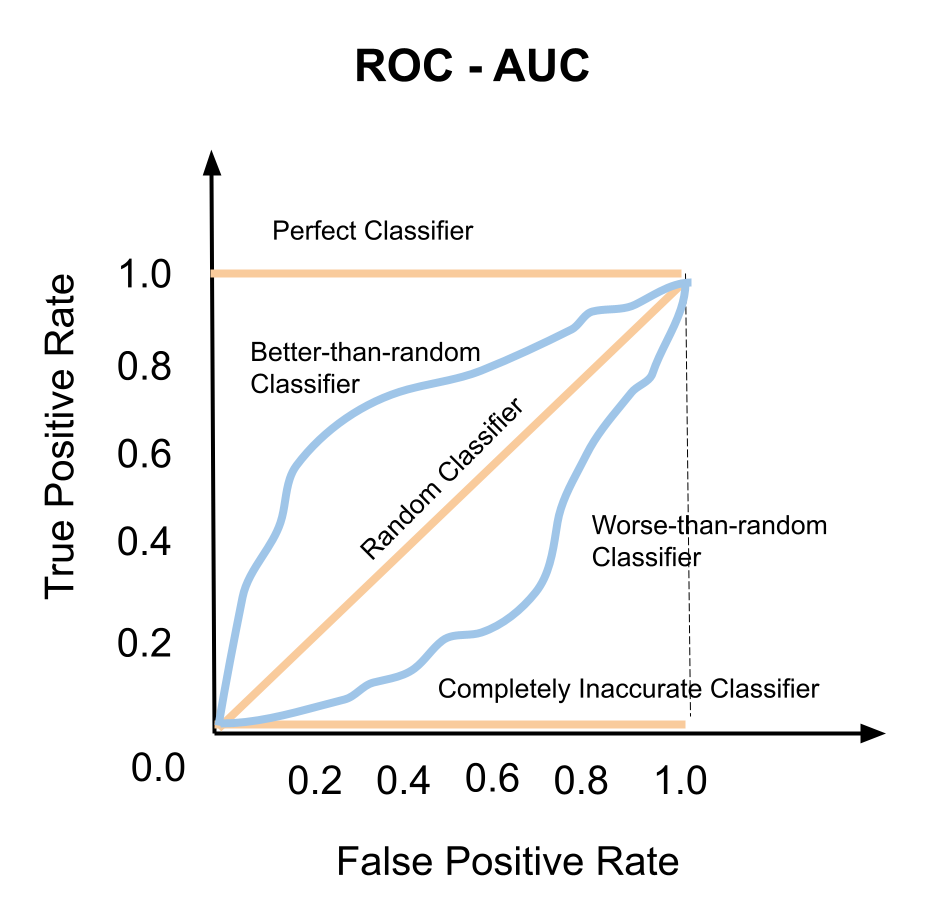
\includegraphics[width=0.5\textwidth]{Figures/02/02_AUC.png}
    \caption{Area Under Curve}
    \label{fig:02_auc}
\end{figure}

The \gls{auc} is simply the area under the ROC curve, and can be used to evaluate probabilistic classifiers, because:

\begin{itemize}
    \item A perfect classifier has an \gls{auc} of 1.0
    \item A completely inaccurate classifier has an \gls{auc} of 0.0
    \item A random classifier has an \gls{auc} of 0.5
    \item A better-than-random classifier has an \gls{auc} above 0.5
    \item A worse-than-random classifier has an \gls{auc} below 0.5
\end{itemize}

